\documentclass[Lecture.tex]{subfiles}
\begin{document}
\section{2.4: Exploring Features of Quantitative Data with Pictures}


\begin{frame}{Example}
Looking at a list of numerical data is about as informative as looking at a page of scrambled letters:
\begin{center}
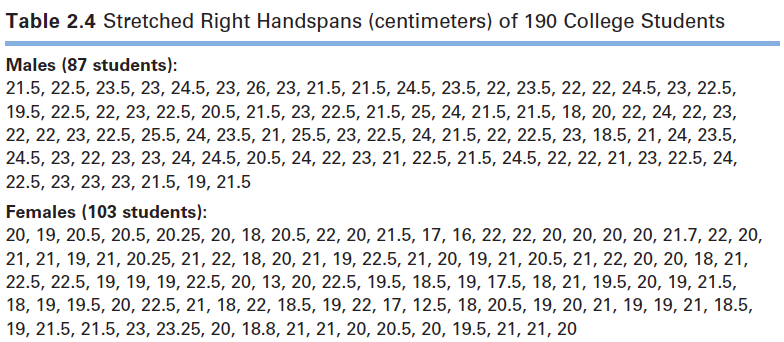
\includegraphics[scale=.4]{handspans}
\end{center}
 \end{frame}

\begin{frame}{Simple Dotplot}
\begin{center}
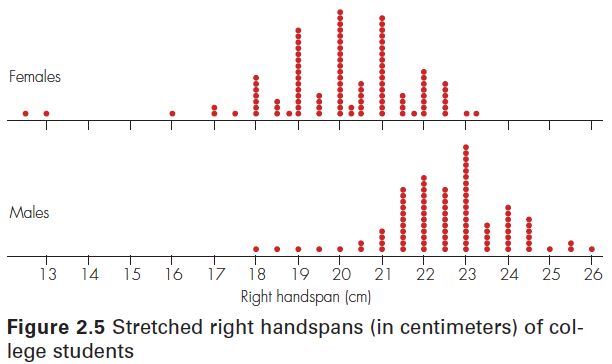
\includegraphics[scale=.5]{handspansdotplot}
\end{center}
\end{frame}

\begin{frame}{Definitions}
\begin{defn}
    \begin{itemize}
    \item<1->
      The {\it distribution} of a quantitative variable is the overall pattern of how often the possible values occur.  There are three summary characteristics that tend to be of most interest:
    \item<2->
      The {\it location} (center, average),
    \item<3->
      the {\it spread} (variability),
    \item<4->
    and the {\it shape} of the data.
    \end{itemize}
  \end{defn}
\end{frame}

\begin{frame}{Location}
There are two common measures for estimating location:
\begin{defn}
   \begin{itemize}
   \item<1->
     The {\it median}, approximately the middle value in the data, and
   \item<2->
     the {\it mean}, which is the usual arithmetic average.
   \end{itemize}
\end{defn}
\end{frame}

\begin{frame}{Spread}
The {\it variability} of a dataset considers how spread out the values are; are they all about the same? are most together but some unusually high or low?  Two ways to assess the spread are
\begin{defn}
\begin{itemize}
\item<1->
  The {\it range} (the difference between the maximum and minimum values) and
\item<2->
  the difference between the two quartiles or the {\it interquartile range}. (The lower and upper quartiles are roughly the medians of the lower and upper halves of ordered data.)
\end{itemize}
\end{defn}
\end{frame}

\begin{frame}{Shape}
Using appropriate visual displays, we can address questions about shape such as: Are most of the values clumped in the middle, with values tailing off to each end? Are most clumped to one side or the other?\pause
\begin{center}
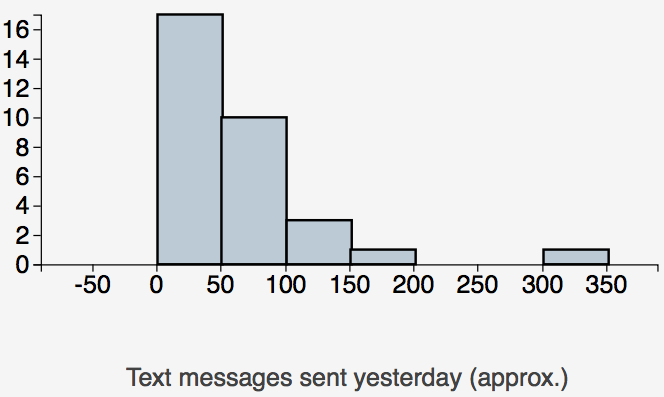
\includegraphics[scale=.3]{shape1}
\end{center}
\end{frame}

\begin{frame}{Shape}
Using appropriate visual displays, we can address questions about shape such as: Are most of the values clumped in the middle, with values tailing off to each end? Are most clumped to one side or the other?
\begin{center}
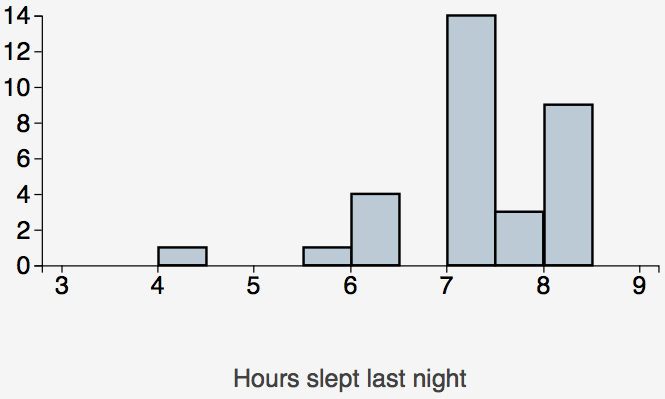
\includegraphics[scale=.3]{shape2}
\end{center}
\end{frame}

\begin{frame}{Outliers}
\begin{defn}
There is no precise definition for an {\it outlier}, but in general, an outlier is a data point that is not consistent with the bulk of the data.\\ \pause
For a single variable, an outlier is a value that is unusually high or low.\\ \pause
When two variables are considered, an outlier is an unusual combination of values.\\ \pause
{\bf Note:} The extreme values do not automatically qualify as outliers.
\end{defn}
\end{frame}

\begin{frame}{Five-number Summary}
We can summarize data using a {\it five-number summary} which includes the median, quartiles, and the extremes.\pause
\begin{center}
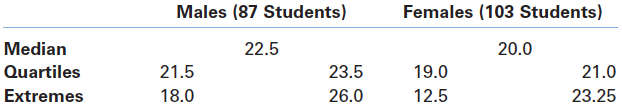
\includegraphics[scale=.4]{handspanssummary}
\end{center}\pause
Compared to the list of raw data, this summary tells us a lot more about the handspans of male and female college students.
\end{frame}

\begin{frame}{Strengths and Weaknesses of Visual Displays}
The types of visual displays we have seen include histograms, stem-and-leaf plots, dotplots, and boxplots.  Each of these displays organizes quantitative data in ways that let us begin to find the information in a dataset.  Which type of display is best depends entirely on the data, what feature of the data may be of interest, and sample size.
\end{frame}

\begin{frame}{Histograms}
\begin{itemize}
\item<1->
  {\it Strengths:} Can quickly determine shape of a moderate to large dataset.  Flexibility in choosing the number as well as the width of the intervals for the display (usually between 6 and 15 intervals gives a good picture).
\item<2->
  {\it Weaknesses:} With a small sample, there may not be enough data to show the shape.  With either too few or too many intervals, we may not see the true shape.
\end{itemize}
\end{frame}
\begin{frame}{Histograms}
\begin{center}
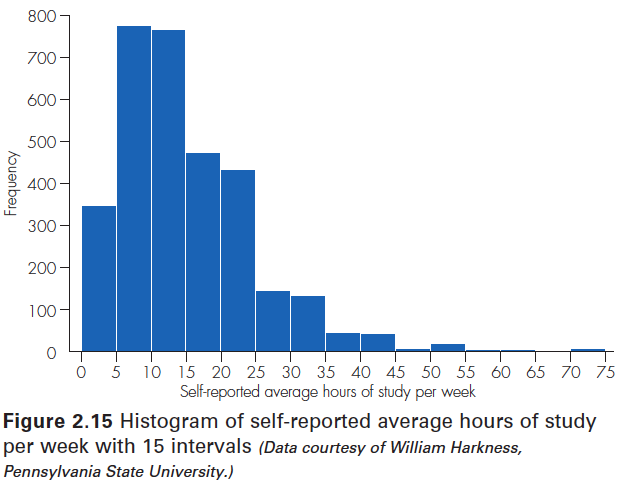
\includegraphics[scale=.4]{histogram1}
\end{center}
\end{frame}

\begin{frame}{Histograms}
\begin{center}
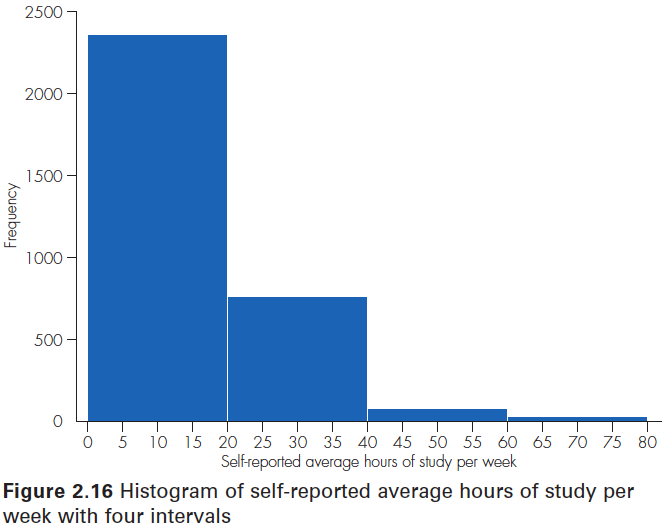
\includegraphics[scale=.4]{histogram2}
\end{center}
\end{frame}

\begin{frame}{Stem-and-Leaf Plots}
\begin{itemize}
\item<1->
  {\it Strengths:} Good for sorting data and with a sufficient sample size, can be used to judge shape.
\item<2->
  {\it Weaknesses:} With a large sample size, a stem-and-leaf plot may be too cluttered since it shows each individual data point.
\end{itemize}
\end{frame}

\begin{frame}{Boxplots}
Boxplots are useful for picturing the information given in one or more five-number summaries and are also useful in identifying outliers.\\ \pause
\begin{itemize}
\item<1->
{\it Strengths:}  Summarize five-number summary, so they give a direct look at location and spread.  Identify outliers.  Easy to compare two or more groups.
\item<2->
{\it Weaknesses:} Not very useful for judging shape.
\end{itemize}
\end{frame}

\begin{frame}{How to Draw a Boxplot}

{\bf 1)}  Label either a vertical axis or horizontal axis with numbers from the minimum to the maximum of the data.\pause

{\bf 2)}  Draw a box with the lower end of the box at the lower quartile (denoted as $Q_1$) and the upper end at the upper quartile ($Q_3$).\pause

{\bf 3)}  Draw a line through the box at the median.\pause

{\bf 4)}  Calculate $IQR=Q_3-Q_1$.\pause

{\bf 5)}  Draw a line that extends from the lower quartile end of the box to the smallest data value not smaller than the value of $Q_1-1.5(IQR)$.  Also, draw a line that extends from the upper quartile end of the box to the largest data value that is not greater than the value of $Q_3+1.5(IQR)$.\pause

{\bf 6)}  Mark the location of any data points smaller than $Q_1-1.5(IQR)$ or larger than $Q_3+1.5(IQR)$ with an asterisk.  These values are considered to be outliers.

%\end{defn}
\end{frame}


\begin{frame}{Example}
The following is a five-number summary based on data gathered regarding number of songs on students' iPods or MP3 players.  
\begin{center}
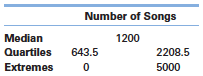
\includegraphics{songs}
\end{center}
\end{frame}








\end{document}
